\documentclass[journal]{IEEEtran}

\usepackage[utf8]{inputenc}
\usepackage{hyperref}
\usepackage{natbib}
\usepackage{todonotes}
\usepackage{color}
\usepackage{svg}
\usepackage{arrayjob}
\usepackage{multirow}


\hypersetup{
    %bookmarks=true,         % show bookmarks bar?
    unicode=false,          % non-Latin characters in Acrobats bookmarks
    pdftoolbar=true,        % show Acrobats toolbar?
    pdfmenubar=true,        % show Acrobats menu?
    pdffitwindow=false,     % window fit to page when opened
    pdfstartview={FitH},    % fits the width of the page to the window
    pdftitle={TDT4501 - Toward a SHMAC ISA and Microarchitecture: An Experimental Approach on the ARM ISA},    % title
    pdfauthor={Stian Hvatum, Terje Runde},     % author
    pdfsubject={Prefetching techniques},   % subject of the document
    pdfcreator={Stian Hvatum, Terje Runde},   % creator of the document
    pdfproducer={Stian Hvatum, Terje Runde}, % producer of the document
    pdfnewwindow=true,      % links in new window
    colorlinks,       % false: boxed links; true: colored links
    linkcolor=black,          % color of internal links
    citecolor=black,        % color of links to bibliography
    filecolor=magenta,      % color of file links
    urlcolor=black           % color of external links
}




\begin{document}

\title{\small{TDT4501 - Toward a SHMAC ISA and Microarchitecture}\\\Huge{An Experimental Approach on the ARM ISA}}

\author{Terje~Runde,~MSc.~CS~student~NTNU,
        Stian~Hvatum,~MSc.~CS~student~NTNU}


\maketitle

\begin{abstract}

This paper investigates the instruction level energy efficency of an Cortex-A9,
and presents numbers on energy comsumption pr. instruction.  The investigation
shows that even though the ARM Cortex-A9 is a computationaly strong and energy
efficient CPU, there are room for improvements.

\end{abstract}


\begin{IEEEkeywords}
Power consumption, ARM, performance counters, instruction level energy efficency
\end{IEEEkeywords}

\section{Introduction}

\IEEEPARstart{M}{oore's} law is very often the first word in a paper about computer science.
This is in fact a paper about computer science, and thus starts with the words Moore's law.

\section{Related work}
Real Time Power Estimation and Thread Scheduling via Performance Counters, Karan Singh, Major Bhadauria, Sally A. McKee, ACM SIGARCH Computer Architecture News archive, May 2009 (ITSL) 

Decomposable and Responsive Power Models for Multi-core Processors using Performance Counters, ICS'10, Ramon Bertran et.al., June 2010. (ITSL)

Complete System Power Estimation Using Processor Performance Events, Bircher and John, IEEE Trans on comput, April 2012 (ITSL)
 % beginning or end?
\section{Description of the ARM Cortex A9 CPU}

% TODO: Terje wants this section to be under Methology

The processor we used in the experiment was an ARM Cortex A9
r3p0\footnote{Revision number revealed by printing the contents of the Main ID
Register}, hereby denoted A9. This processor runs at a static frequency of
1.7GHz, have 4 32-bit cores, each with its own out-of-order dual issue
speculative pipelines\cite{armtech}. The pipeline is split after the dispatch
stage into 4 different lines, each with its own functional units. The different
pipelines is not very well documented, but our experiments together with the
common subset of information found in various
documentations\cite{armtech}\cite{7cpu}\cite{lotofdocs}, the four pipelines are
structured as follow: Main execution pipeline with a  general ALU, and a
hardware-multiply, secondary execution pipeline with only a general ALU,
load-store-pipeline, containing only an hardware adder to generate addresses,
and a floating-point pipeline containing an ordinary FPU and connections to the
NEON unit.

It is a common philosophy that a RISC should consume one clock cycle pr.
instruction\cite{unknown}.  For this particular processor made by Advanced RISC
Machines, it is not the case. The dual issue and its parallel general ALU
pipelines enables the processor to achieve more than one instruction pr. clock
cycle, and at the same time, it supports multiply, divide and floating point,
each taking multiple clock cycles. It is even so that multiply, divide and
floating point takes different amount of cycles according to their surrounding
instructions.

The A9 processor contains an Performance Monitor Unit with 6 generic event
counters, a cycle counter and 58 different events that are mappable to the event
counters\cite{armtech}. A list of possible events can be found in table A.18 in
the Cortex-A9 Technical Reference Manual\cite{armtech}.



\section{ISA Dependent Energy Consumption}
% General approach here? Implementation in methodology? Order of appearance?

\todo[inline]{Give some background on what exactly burns energy in a processor.
Be as precise as possible -- dissect the pipeline.}
Since this paper investigates the ISA dependent power consumption, we do not
look into the details of components other that the CPU core. In some
architectures, cache and other components close to the core are driven by the
same supply rail\cite{rusu200765}. We try to disable or avoid usage of such
components as much as possible.


This method mainly focuses on comparison between instructions, and the energy
consumption of the condition calculation and the conditional jump can then be
seen as part of the common baseline.
\todo[inline]{Correct assumption? Probably. Explain why we need a baseline
instruction.}

\begin{figure}
    % Graphic for TeX using PGF
% Title: /home/hvatum/Skole/arm-project/report/figures/setup.xml
% Creator: Dia v0.97.2
% CreationDate: Tue Nov 19 12:35:36 2013
% For: hvatum
% \usepackage{tikz}
% The following commands are not supported in PSTricks at present
% We define them conditionally, so when they are implemented,
% this pgf file will use them.
\ifx\du\undefined
  \newlength{\du}
\fi
\setlength{\du}{15\unitlength}
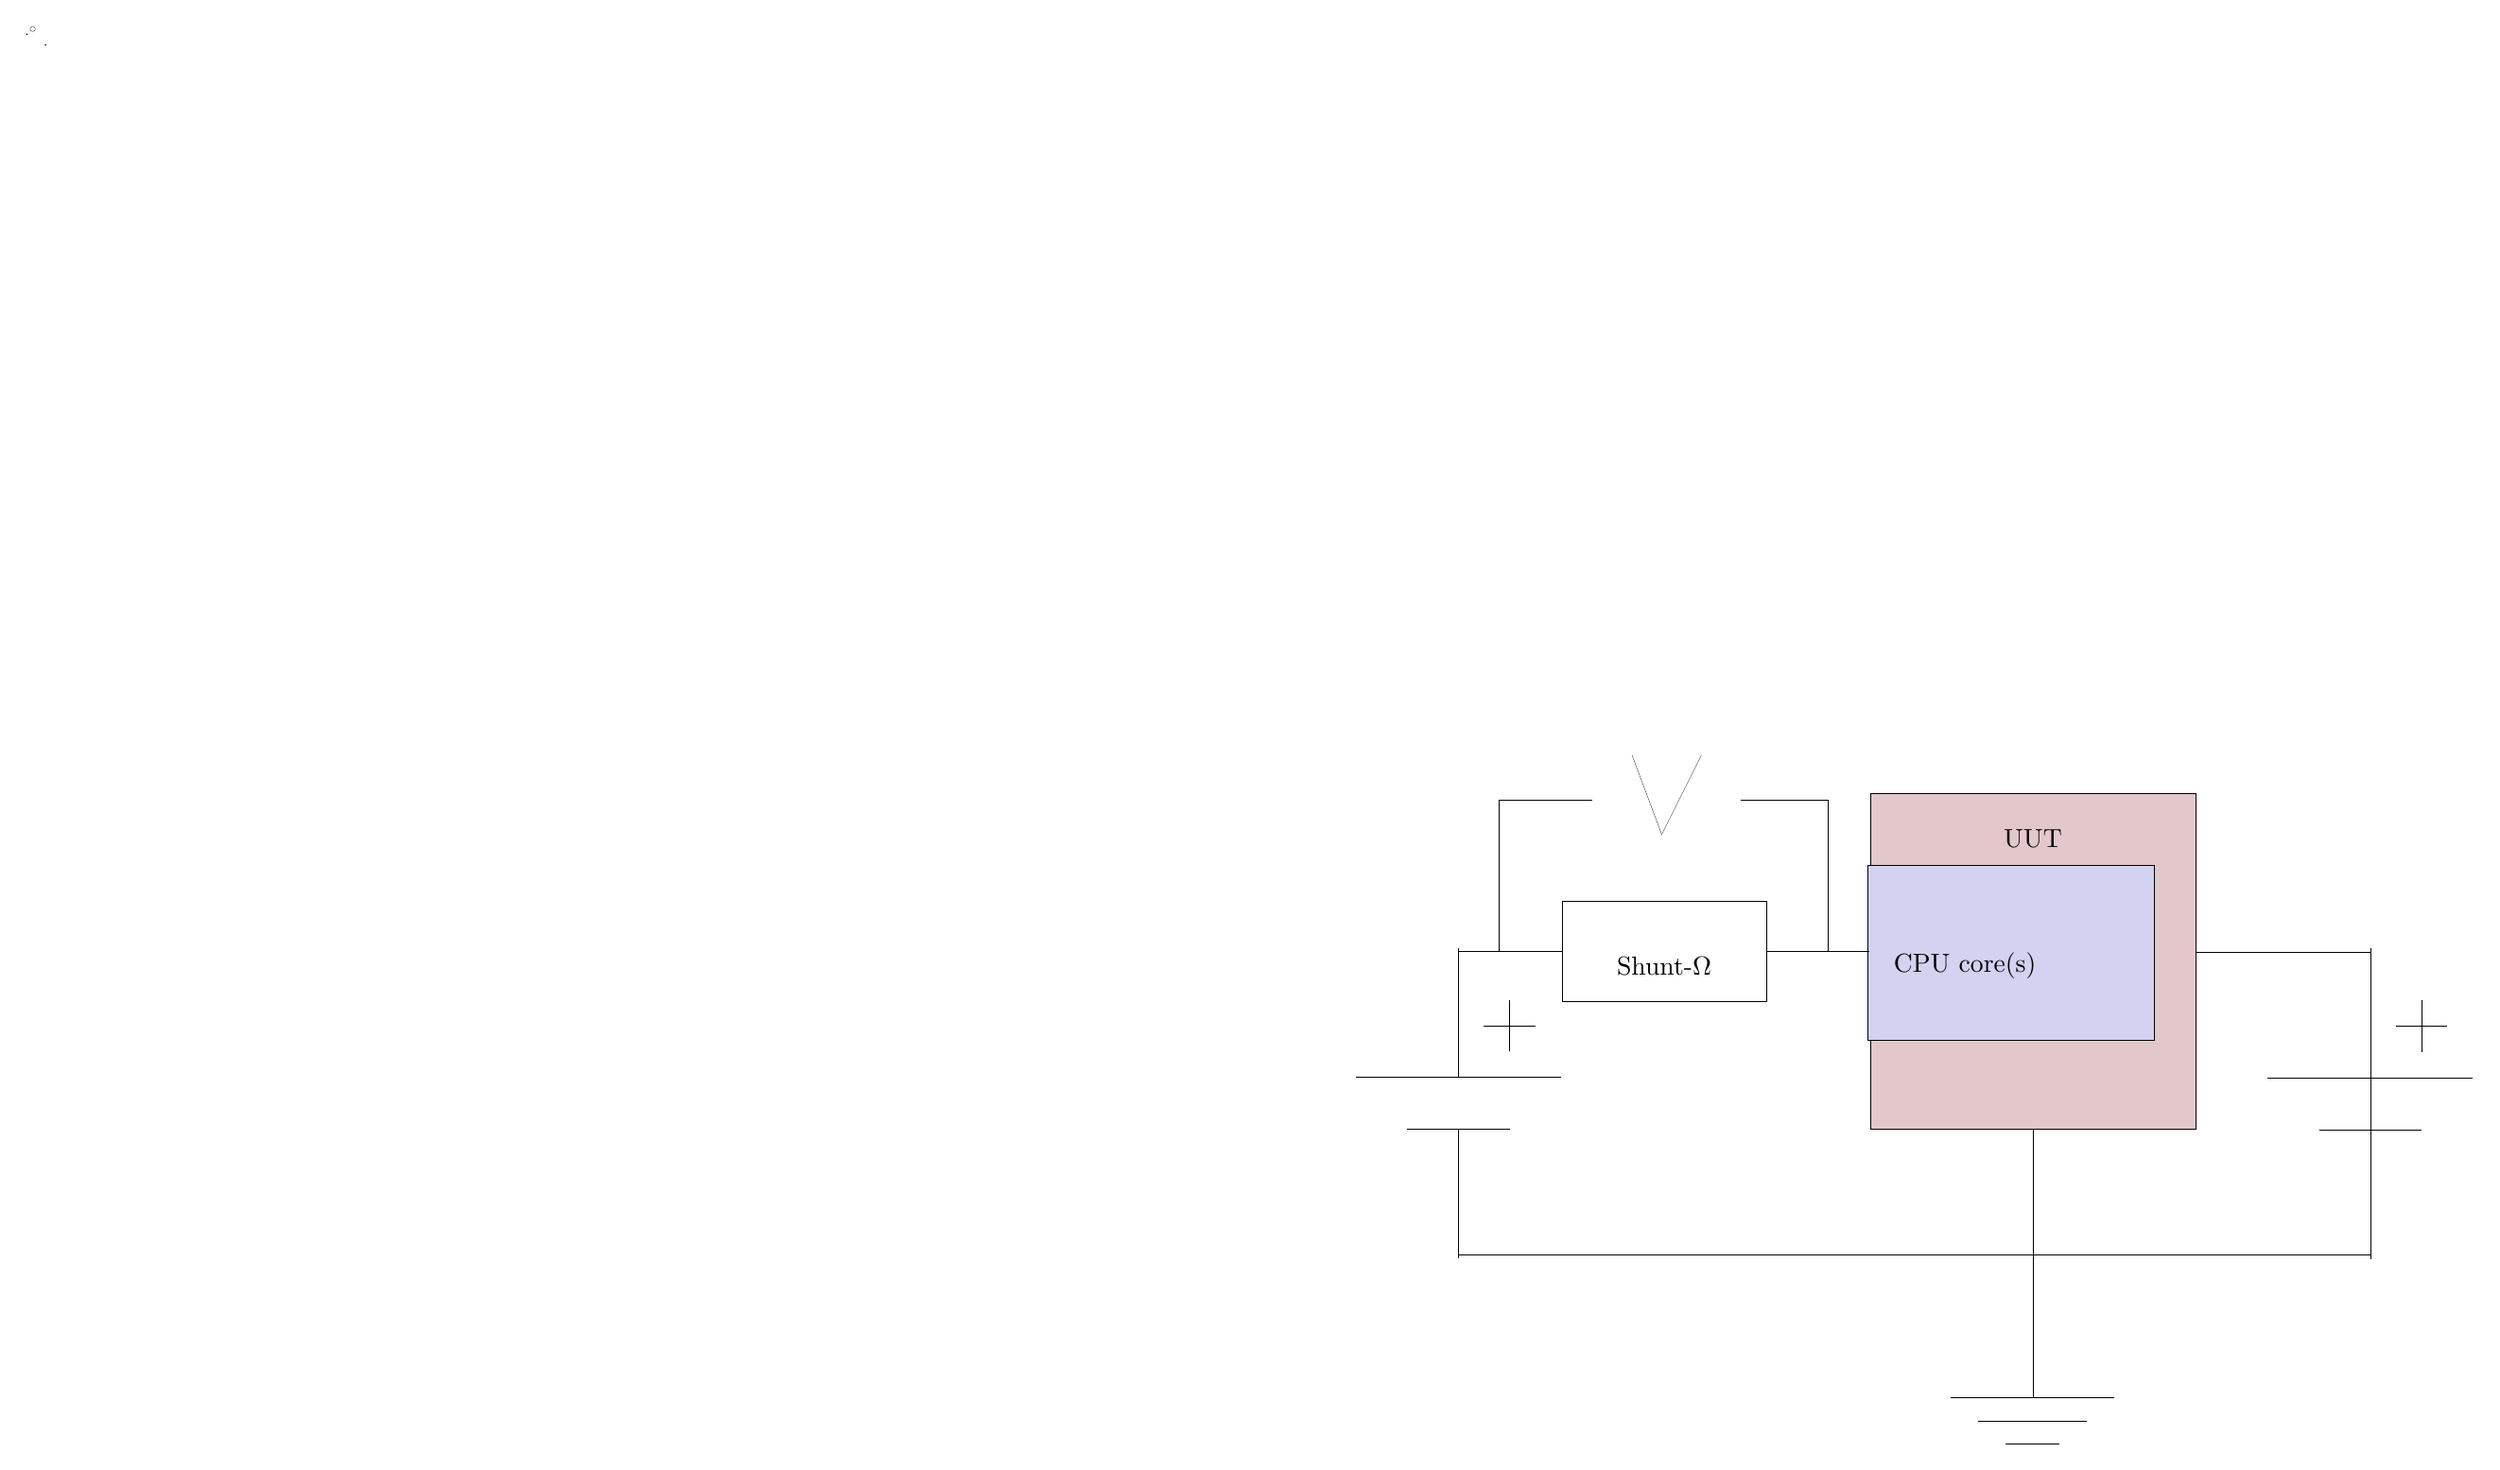
\begin{tikzpicture}
\pgftransformxscale{1.000000}
\pgftransformyscale{-1.000000}
\definecolor{dialinecolor}{rgb}{0.000000, 0.000000, 0.000000}
\pgfsetstrokecolor{dialinecolor}
\definecolor{dialinecolor}{rgb}{1.000000, 1.000000, 1.000000}
\pgfsetfillcolor{dialinecolor}
\pgfsetlinewidth{0.100000\du}
\pgfsetdash{}{0pt}
\pgfsetdash{}{0pt}
\pgfsetbuttcap
\pgfsetmiterjoin
\pgfsetlinewidth{0.100000\du}
\pgfsetbuttcap
\pgfsetmiterjoin
\pgfsetdash{}{0pt}
\definecolor{dialinecolor}{rgb}{0.000000, 0.000000, 0.000000}
\pgfsetstrokecolor{dialinecolor}
\draw (19.962100\du,12.768751\du)--(21.337939\du,12.768751\du);
\pgfsetbuttcap
\pgfsetmiterjoin
\pgfsetdash{}{0pt}
\definecolor{dialinecolor}{rgb}{1.000000, 1.000000, 1.000000}
\pgfsetfillcolor{dialinecolor}
\fill (21.337939\du,12.097000\du)--(21.337939\du,13.440503\du)--(24.089616\du,13.440503\du)--(24.089616\du,12.097000\du)--cycle;
\definecolor{dialinecolor}{rgb}{0.000000, 0.000000, 0.000000}
\pgfsetstrokecolor{dialinecolor}
\draw (21.337939\du,12.097000\du)--(21.337939\du,13.440503\du)--(24.089616\du,13.440503\du)--(24.089616\du,12.097000\du)--cycle;
\pgfsetbuttcap
\pgfsetmiterjoin
\pgfsetdash{}{0pt}
\definecolor{dialinecolor}{rgb}{0.000000, 0.000000, 0.000000}
\pgfsetstrokecolor{dialinecolor}
\draw (24.089616\du,12.768751\du)--(25.465455\du,12.768751\du);
\pgfsetlinewidth{0.100000\du}
\pgfsetdash{}{0pt}
\pgfsetdash{}{0pt}
\pgfsetbuttcap
\pgfsetmiterjoin
\pgfsetlinewidth{0.100000\du}
\pgfsetbuttcap
\pgfsetmiterjoin
\pgfsetdash{}{0pt}
\definecolor{dialinecolor}{rgb}{0.890196, 0.784314, 0.796078}
\pgfsetfillcolor{dialinecolor}
\fill (25.484300\du,10.640900\du)--(25.484300\du,15.148903\du)--(29.846883\du,15.148903\du)--(29.846883\du,10.640900\du)--cycle;
\definecolor{dialinecolor}{rgb}{0.000000, 0.000000, 0.000000}
\pgfsetstrokecolor{dialinecolor}
\draw (25.484300\du,10.640900\du)--(25.484300\du,15.148903\du)--(29.846883\du,15.148903\du)--(29.846883\du,10.640900\du)--cycle;
\pgfsetbuttcap
\pgfsetmiterjoin
\pgfsetdash{}{0pt}
\definecolor{dialinecolor}{rgb}{0.000000, 0.000000, 0.000000}
\pgfsetstrokecolor{dialinecolor}
\draw (25.484300\du,10.640900\du)--(25.484300\du,15.148903\du)--(29.846883\du,15.148903\du)--(29.846883\du,10.640900\du)--cycle;
\pgfsetlinewidth{0.100000\du}
\pgfsetdash{}{0pt}
\pgfsetdash{}{0pt}
\pgfsetmiterjoin
\definecolor{dialinecolor}{rgb}{0.827451, 0.823529, 0.941176}
\pgfsetfillcolor{dialinecolor}
\fill (25.440800\du,11.611400\du)--(25.440800\du,13.961400\du)--(29.291289\du,13.961400\du)--(29.291289\du,11.611400\du)--cycle;
\definecolor{dialinecolor}{rgb}{0.000000, 0.000000, 0.000000}
\pgfsetstrokecolor{dialinecolor}
\draw (25.440800\du,11.611400\du)--(25.440800\du,13.961400\du)--(29.291289\du,13.961400\du)--(29.291289\du,11.611400\du)--cycle;
% setfont left to latex
\definecolor{dialinecolor}{rgb}{0.000000, 0.000000, 0.000000}
\pgfsetstrokecolor{dialinecolor}
\node[anchor=west] at (25.677700\du,12.964800\du){CPU core(s)};
\pgfsetlinewidth{0.100000\du}
\pgfsetdash{}{0pt}
\pgfsetdash{}{0pt}
\pgfsetbuttcap
\pgfsetmiterjoin
\pgfsetlinewidth{0.100000\du}
\pgfsetbuttcap
\pgfsetmiterjoin
\pgfsetdash{}{0pt}
\definecolor{dialinecolor}{rgb}{0.000000, 0.000000, 0.000000}
\pgfsetstrokecolor{dialinecolor}
\draw (27.664452\du,18.153700\du)--(27.664452\du,18.766668\du);
\pgfsetbuttcap
\pgfsetmiterjoin
\pgfsetdash{}{0pt}
\definecolor{dialinecolor}{rgb}{0.000000, 0.000000, 0.000000}
\pgfsetstrokecolor{dialinecolor}
\draw (26.565900\du,18.766668\du)--(28.763005\du,18.766668\du);
\pgfsetbuttcap
\pgfsetmiterjoin
\pgfsetdash{}{0pt}
\definecolor{dialinecolor}{rgb}{0.000000, 0.000000, 0.000000}
\pgfsetstrokecolor{dialinecolor}
\draw (26.933915\du,19.073151\du)--(28.394990\du,19.073151\du);
\pgfsetbuttcap
\pgfsetmiterjoin
\pgfsetdash{}{0pt}
\definecolor{dialinecolor}{rgb}{0.000000, 0.000000, 0.000000}
\pgfsetstrokecolor{dialinecolor}
\draw (27.301930\du,19.379635\du)--(28.026975\du,19.379635\du);
% setfont left to latex
\definecolor{dialinecolor}{rgb}{0.000000, 0.000000, 0.000000}
\pgfsetstrokecolor{dialinecolor}
\node at (22.713800\du,12.972644\du){Shunt-$\Omega$};
\pgfsetlinewidth{0.100000\du}
\pgfsetdash{}{0pt}
\pgfsetdash{}{0pt}
\pgfsetbuttcap
\pgfsetmiterjoin
\pgfsetlinewidth{0.100000\du}
\pgfsetbuttcap
\pgfsetmiterjoin
\pgfsetdash{}{0pt}
\definecolor{dialinecolor}{rgb}{1.000000, 1.000000, 1.000000}
\pgfsetfillcolor{dialinecolor}
\pgfpathellipse{\pgfpoint{22.747033\du}{10.732410\du}}{\pgfpoint{1.000000\du}{0\du}}{\pgfpoint{0\du}{1.000000\du}}
\pgfusepath{fill}
\definecolor{dialinecolor}{rgb}{0.000000, 0.000000, 0.000000}
\pgfsetstrokecolor{dialinecolor}
\pgfpathellipse{\pgfpoint{22.747033\du}{10.732410\du}}{\pgfpoint{1.000000\du}{0\du}}{\pgfpoint{0\du}{1.000000\du}}
\pgfusepath{stroke}
\pgfsetbuttcap
\pgfsetmiterjoin
\pgfsetdash{}{0pt}
\definecolor{dialinecolor}{rgb}{0.000000, 0.000000, 0.000000}
\pgfsetstrokecolor{dialinecolor}
\draw (22.680367\du,11.199077\du)--(23.213700\du,10.132410\du);
\pgfsetbuttcap
\pgfsetmiterjoin
\pgfsetdash{}{0pt}
\definecolor{dialinecolor}{rgb}{0.000000, 0.000000, 0.000000}
\pgfsetstrokecolor{dialinecolor}
\draw (22.680367\du,11.199077\du)--(22.280367\du,10.132410\du);
\pgfsetbuttcap
\pgfsetmiterjoin
\pgfsetdash{}{0pt}
\definecolor{dialinecolor}{rgb}{0.000000, 0.000000, 0.000000}
\pgfsetstrokecolor{dialinecolor}
\draw (20.613700\du,10.732410\du)--(21.747033\du,10.732410\du);
\pgfsetbuttcap
\pgfsetmiterjoin
\pgfsetdash{}{0pt}
\definecolor{dialinecolor}{rgb}{0.000000, 0.000000, 0.000000}
\pgfsetstrokecolor{dialinecolor}
\draw (23.747033\du,10.732410\du)--(24.880367\du,10.732410\du);
\pgfsetlinewidth{0.100000\du}
\pgfsetdash{}{0pt}
\pgfsetdash{}{0pt}
\pgfsetbuttcap
\pgfsetmiterjoin
\pgfsetlinewidth{0.100000\du}
\pgfsetbuttcap
\pgfsetmiterjoin
\pgfsetdash{}{0pt}
\definecolor{dialinecolor}{rgb}{0.000000, 0.000000, 0.000000}
\pgfsetstrokecolor{dialinecolor}
\draw (32.197597\du,12.729500\du)--(32.197597\du,14.467068\du);
\pgfsetbuttcap
\pgfsetmiterjoin
\pgfsetdash{}{0pt}
\definecolor{dialinecolor}{rgb}{0.000000, 0.000000, 0.000000}
\pgfsetstrokecolor{dialinecolor}
\draw (30.819800\du,14.467068\du)--(33.575394\du,14.467068\du);
\pgfsetbuttcap
\pgfsetmiterjoin
\pgfsetdash{}{0pt}
\definecolor{dialinecolor}{rgb}{0.000000, 0.000000, 0.000000}
\pgfsetstrokecolor{dialinecolor}
\draw (31.508699\du,15.162095\du)--(32.886496\du,15.162095\du);
\pgfsetbuttcap
\pgfsetmiterjoin
\pgfsetdash{}{0pt}
\definecolor{dialinecolor}{rgb}{0.000000, 0.000000, 0.000000}
\pgfsetstrokecolor{dialinecolor}
\draw (32.886496\du,13.424527\du)--(32.886496\du,14.119554\du);
\pgfsetbuttcap
\pgfsetmiterjoin
\pgfsetdash{}{0pt}
\definecolor{dialinecolor}{rgb}{0.000000, 0.000000, 0.000000}
\pgfsetstrokecolor{dialinecolor}
\draw (32.542046\du,13.772041\du)--(33.230945\du,13.772041\du);
\pgfsetbuttcap
\pgfsetmiterjoin
\pgfsetdash{}{0pt}
\definecolor{dialinecolor}{rgb}{0.000000, 0.000000, 0.000000}
\pgfsetstrokecolor{dialinecolor}
\draw (32.197597\du,15.162095\du)--(32.197597\du,16.899662\du);
\pgfsetlinewidth{0.100000\du}
\pgfsetdash{}{0pt}
\pgfsetdash{}{0pt}
\pgfsetbuttcap
\pgfsetmiterjoin
\pgfsetlinewidth{0.100000\du}
\pgfsetbuttcap
\pgfsetmiterjoin
\pgfsetdash{}{0pt}
\definecolor{dialinecolor}{rgb}{0.000000, 0.000000, 0.000000}
\pgfsetstrokecolor{dialinecolor}
\draw (19.947397\du,12.724100\du)--(19.947397\du,14.461668\du);
\pgfsetbuttcap
\pgfsetmiterjoin
\pgfsetdash{}{0pt}
\definecolor{dialinecolor}{rgb}{0.000000, 0.000000, 0.000000}
\pgfsetstrokecolor{dialinecolor}
\draw (18.569600\du,14.461668\du)--(21.325194\du,14.461668\du);
\pgfsetbuttcap
\pgfsetmiterjoin
\pgfsetdash{}{0pt}
\definecolor{dialinecolor}{rgb}{0.000000, 0.000000, 0.000000}
\pgfsetstrokecolor{dialinecolor}
\draw (19.258499\du,15.156695\du)--(20.636296\du,15.156695\du);
\pgfsetbuttcap
\pgfsetmiterjoin
\pgfsetdash{}{0pt}
\definecolor{dialinecolor}{rgb}{0.000000, 0.000000, 0.000000}
\pgfsetstrokecolor{dialinecolor}
\draw (20.636296\du,13.419127\du)--(20.636296\du,14.114154\du);
\pgfsetbuttcap
\pgfsetmiterjoin
\pgfsetdash{}{0pt}
\definecolor{dialinecolor}{rgb}{0.000000, 0.000000, 0.000000}
\pgfsetstrokecolor{dialinecolor}
\draw (20.291846\du,13.766641\du)--(20.980745\du,13.766641\du);
\pgfsetbuttcap
\pgfsetmiterjoin
\pgfsetdash{}{0pt}
\definecolor{dialinecolor}{rgb}{0.000000, 0.000000, 0.000000}
\pgfsetstrokecolor{dialinecolor}
\draw (19.947397\du,15.156695\du)--(19.947397\du,16.894262\du);
\pgfsetlinewidth{0.100000\du}
\pgfsetdash{}{0pt}
\pgfsetdash{}{0pt}
\pgfsetmiterjoin
\pgfsetbuttcap
{
\definecolor{dialinecolor}{rgb}{0.000000, 0.000000, 0.000000}
\pgfsetfillcolor{dialinecolor}
% was here!!!
{\pgfsetcornersarced{\pgfpoint{0.000000\du}{0.000000\du}}\definecolor{dialinecolor}{rgb}{0.000000, 0.000000, 0.000000}
\pgfsetstrokecolor{dialinecolor}
\draw (29.846900\du,12.894900\du)--(29.846900\du,12.780100\du)--(32.197597\du,12.780100\du)--(32.197597\du,14.814581\du);
}}
\pgfsetlinewidth{0.100000\du}
\pgfsetdash{}{0pt}
\pgfsetdash{}{0pt}
\pgfsetmiterjoin
\pgfsetbuttcap
{
\definecolor{dialinecolor}{rgb}{0.000000, 0.000000, 0.000000}
\pgfsetfillcolor{dialinecolor}
% was here!!!
{\pgfsetcornersarced{\pgfpoint{0.000000\du}{0.000000\du}}\definecolor{dialinecolor}{rgb}{0.000000, 0.000000, 0.000000}
\pgfsetstrokecolor{dialinecolor}
\draw (19.947400\du,15.988800\du)--(19.947400\du,16.842000\du)--(27.664400\du,16.842000\du)--(27.664400\du,18.153700\du);
}}
\pgfsetlinewidth{0.100000\du}
\pgfsetdash{}{0pt}
\pgfsetdash{}{0pt}
\pgfsetmiterjoin
\pgfsetbuttcap
{
\definecolor{dialinecolor}{rgb}{0.000000, 0.000000, 0.000000}
\pgfsetfillcolor{dialinecolor}
% was here!!!
{\pgfsetcornersarced{\pgfpoint{0.000000\du}{0.000000\du}}\definecolor{dialinecolor}{rgb}{0.000000, 0.000000, 0.000000}
\pgfsetstrokecolor{dialinecolor}
\draw (27.664400\du,18.153700\du)--(27.664400\du,16.848900\du)--(32.197597\du,16.848900\du)--(32.197597\du,14.814581\du);
}}
\pgfsetlinewidth{0.100000\du}
\pgfsetdash{}{0pt}
\pgfsetdash{}{0pt}
\pgfsetmiterjoin
\pgfsetbuttcap
{
\definecolor{dialinecolor}{rgb}{0.000000, 0.000000, 0.000000}
\pgfsetfillcolor{dialinecolor}
% was here!!!
{\pgfsetcornersarced{\pgfpoint{0.000000\du}{0.000000\du}}\definecolor{dialinecolor}{rgb}{0.000000, 0.000000, 0.000000}
\pgfsetstrokecolor{dialinecolor}
\draw (21.462300\du,10.732400\du)--(20.492500\du,10.732400\du)--(20.492500\du,12.768800\du)--(20.810700\du,12.768800\du);
}}
\pgfsetlinewidth{0.100000\du}
\pgfsetdash{}{0pt}
\pgfsetdash{}{0pt}
\pgfsetmiterjoin
\pgfsetbuttcap
{
\definecolor{dialinecolor}{rgb}{0.000000, 0.000000, 0.000000}
\pgfsetfillcolor{dialinecolor}
% was here!!!
{\pgfsetcornersarced{\pgfpoint{0.000000\du}{0.000000\du}}\definecolor{dialinecolor}{rgb}{0.000000, 0.000000, 0.000000}
\pgfsetstrokecolor{dialinecolor}
\draw (24.880400\du,10.732400\du)--(24.911900\du,10.732400\du)--(24.911900\du,12.768800\du)--(25.465500\du,12.768800\du);
}}
\pgfsetlinewidth{0.100000\du}
\pgfsetdash{}{0pt}
\pgfsetdash{}{0pt}
\pgfsetmiterjoin
\pgfsetbuttcap
{
\definecolor{dialinecolor}{rgb}{0.000000, 0.000000, 0.000000}
\pgfsetfillcolor{dialinecolor}
% was here!!!
{\pgfsetcornersarced{\pgfpoint{0.000000\du}{0.000000\du}}\definecolor{dialinecolor}{rgb}{0.000000, 0.000000, 0.000000}
\pgfsetstrokecolor{dialinecolor}
\draw (27.665592\du,15.148903\du)--(27.665592\du,16.651301\du)--(27.664452\du,16.651301\du)--(27.664452\du,18.153700\du);
}}
% setfont left to latex
\definecolor{dialinecolor}{rgb}{0.000000, 0.000000, 0.000000}
\pgfsetstrokecolor{dialinecolor}
\node at (27.665600\du,11.250900\du){UUT};
\pgfsetlinewidth{0.100000\du}
\pgfsetdash{}{0pt}
\pgfsetdash{}{0pt}
\pgfsetbuttcap
\pgfsetmiterjoin
\pgfsetlinewidth{0.100000\du}
\pgfsetbuttcap
\pgfsetmiterjoin
\pgfsetdash{}{0pt}
\definecolor{dialinecolor}{rgb}{0.000000, 0.000000, 0.000000}
\pgfsetfillcolor{dialinecolor}
\pgfpathellipse{\pgfpoint{27.662690\du}{16.839990\du}}{\pgfpoint{0.191690\du}{0\du}}{\pgfpoint{0\du}{0.191690\du}}
\pgfusepath{fill}
\definecolor{dialinecolor}{rgb}{0.000000, 0.000000, 0.000000}
\pgfsetstrokecolor{dialinecolor}
\pgfpathellipse{\pgfpoint{27.662690\du}{16.839990\du}}{\pgfpoint{0.191690\du}{0\du}}{\pgfpoint{0\du}{0.191690\du}}
\pgfusepath{stroke}
\pgfsetlinewidth{0.010000\du}
\pgfsetbuttcap
\pgfsetmiterjoin
\pgfsetdash{}{0pt}
\definecolor{dialinecolor}{rgb}{0.000000, 0.000000, 0.000000}
\pgfsetstrokecolor{dialinecolor}
\pgfpathellipse{\pgfpoint{27.662690\du}{16.839990\du}}{\pgfpoint{0.191690\du}{0\du}}{\pgfpoint{0\du}{0.191690\du}}
\pgfusepath{stroke}
\pgfsetlinewidth{0.100000\du}
\pgfsetdash{}{0pt}
\pgfsetdash{}{0pt}
\pgfsetbuttcap
\pgfsetmiterjoin
\pgfsetlinewidth{0.100000\du}
\pgfsetbuttcap
\pgfsetmiterjoin
\pgfsetdash{}{0pt}
\definecolor{dialinecolor}{rgb}{0.000000, 0.000000, 0.000000}
\pgfsetfillcolor{dialinecolor}
\pgfpathellipse{\pgfpoint{20.504190\du}{12.767190\du}}{\pgfpoint{0.191690\du}{0\du}}{\pgfpoint{0\du}{0.191690\du}}
\pgfusepath{fill}
\definecolor{dialinecolor}{rgb}{0.000000, 0.000000, 0.000000}
\pgfsetstrokecolor{dialinecolor}
\pgfpathellipse{\pgfpoint{20.504190\du}{12.767190\du}}{\pgfpoint{0.191690\du}{0\du}}{\pgfpoint{0\du}{0.191690\du}}
\pgfusepath{stroke}
\pgfsetlinewidth{0.010000\du}
\pgfsetbuttcap
\pgfsetmiterjoin
\pgfsetdash{}{0pt}
\definecolor{dialinecolor}{rgb}{0.000000, 0.000000, 0.000000}
\pgfsetstrokecolor{dialinecolor}
\pgfpathellipse{\pgfpoint{20.504190\du}{12.767190\du}}{\pgfpoint{0.191690\du}{0\du}}{\pgfpoint{0\du}{0.191690\du}}
\pgfusepath{stroke}
\end{tikzpicture}

    \caption{Experiment Setup}
    \label{fig:setup}
\end{figure}



\section{Methodology}


\subsection{Test Environment}
In our tests, we were using the ODROID-X2 \cite{odroid-x2} developer platform ,
which has an Exynos 4412 "Prime" System-on-Chip with four ARM Cortex-A9 (r3p0) 
processor cores. For all experiments subsequently presented, we disable three of
the cores (1 through 3), leaving only core 0 set to run at a static frequency of
$1.7$ GHz.

The Cortex-A9 is a 32-bit out-of-order dual-issue speculative RISC processor
with many features common for modern processor designs, making it attractive for
our experiments. After the dispatch stage, its pipeline is split into four
different lanes, each with its own functional units. The different pipelines is
not very well documented, but our experiments together with the common subset of
information found in various documentations
\cite{armtech}\cite{7cpu}\cite{lotofdocs}, the four pipelines are structured as
follow: Main execution pipeline with a general ALU, and a hardware-multiply,
secondary execution pipeline with only a general ALU, load-store-pipeline,
containing only an hardware adder to generate addresses, and a floating-point
pipeline containing an ordinary FPU and connections to the NEON unit.

The A9 processor has 58 distinct events that each can be mapped to one of six
generic event counters in the Performance Monitor Unit (i.e. only six generic
events can be tracked simultaneously). It also has a separate cycle counter. A
complete overview can be seen in table $A.18$ in the Cortex-A9 Technical
Reference Manual \cite{armtech}.


\todo[inline]{Move and rewrite this paragraph.}
It is a common philosophy that a RISC should consume one clock cycle pr.
instruction\cite{unknown}. For this particular processor made by Advanced RISC
Machines, it is not the case. The dual issue and its parallell general ALU
pipelines enables the processor to achive more than one instruction pr. clock
cycle, and at the same time, it supports multiply, divide and floating point,
each taking multiple clock cycles. It is even so that multiply, divide and
floating point takes different amount of cycles according to their surrounding
instructions.


\subsection{Architectural Experiments}
\label{arch_experiments}
Running the processor at it's highest possible throughput requires knowledge of
internal components in the pipeline, e.g. to find out the number of $add$s it is
capable of doing per cycle. As we are using a proprietary platform as our target
architecture, only some of these details are known. Thus, we define test
programs to stress particular pipeline components and gather statistics using
performance counters. By comparing execution unit counters and the total cycle
count, we obtain detailed (although approximate, due to the speculativity in the
core) information of a test program's execution.
\todo[inline]{Elaborate in detail, see notes/alu-count.txt.}

Using the same approach as above, we are able to identify a feature on the A9
processor that is very vaguely documented; fast-loop\texttrademark mode. As the
name suggests, this feature enables rapid execution of small loops by bypassing
the L1 cache.  However, which loops that falls into this category is not
documented, but by using performance counters we are able to determine this with
confidence.
\todo[inline]{Add appendix explaining fast-loop microbenchmark.}


\subsection{Benchmarks}
As a first approximation, the benchmark programs consists of an infinite series
of identic instructions. The A9 core runs at a fixed frequency and we are
providing a fixed core voltage, so energy usage of simple, one-cycle instruction
could be retrieved by running for a fixed time period and applying the following
formula.

\todo{fix formula}
\begin{equation}
    P_{instruction} = A_{instruction} \cdot V_{core}
\end{equation}
\begin{equation}
    E_{instruction} = P_{instruction} \cdot CPI_{instruction}
\end{equation}
The Agilent multimeter is set up to sample at full precision at its maximum rate
of 1000 Hz. This yields one sample every $\frac{ f_{core} }{ 1000 } = 1.7$
million instructions; it is obvious from this that we are unable to observe
inter-cycle variations in energy consumption.
\todo[inline]{But maybe the multimeter is doing a running average internally?}

This simple setup does not take the memory system into account; we are
undoubtedly not able to feed the processor instructions at no cost in terms of
access speed and -- more importantly -- memory system energy usage. Thus, we
improve this model by investigating features that avoids the memory system as
much as possible.

Furthermore, executing code within fast-loop allows us to limit the number of
cache mispredicts to 2, independently of the iteration count.
\todo[inline]{Explain how and why these to misses occur}


\subsection{Power Measurements}
To measure energy consumption, we use an Agilent 34410A multimeter and measures
voltage drop over a negligible $12$ $m\Omega$ resistor. We decouple power
consumption on the ARM cores and the development board by modifying the
ODROID-X2 and providing a separate power supply for the A9 cores. They get
powered by an external power supply giving $1.3V$ DC, while the rest of the
board is powered from a another power supply at $5.0V$, as depicted in figure
\todo{figure ref}.

\subsection{Pit Falls}
% temperature, noise (inducted power, etc.), interrupts, memory latency (fast-loop)
Since we are comparing the energy efficency of different instruction in an asynchronous
way, we have to consider factors that affects power usage, as well as acknowledege that
they may differ between runs.

One obviuos such factor is temperature, both ambient and
the chip temperature. The first may change without our notice, and the second one is
determined by the ambient, the cooling device and what load tasks that was just run on
the SoC. On this specific SoC, Samsung Exynos 4412, we have detected that the difference
from the CPU Thermal Zone 0 being 9$^\circ$ Celcius and 63$^\circ$ Celcius is on average
between 2-4\%. We also detected that some instructions might have as much as 7\% higher
energy consumption when running at the hotter level\footnote{This was detected with at
the {\ttfamily mul}-instruction}. We have also checked that running a single core at
maximum performace over time does not increase the temperature by more than from
idle at 47$^\circ$ Celcius to 54$^\circ$ Celcius at load. Assuming that it is generally
true that a single core cannot heat the entire SoC with any significant amount, and that
the increase in power consumption is at max 10\% over 50$^\circ$ Celcius, we get
\begin{equation}
    P_{inc} = P_{orig} \cdot T_{inc} \cdot \frac{0.10}{50} = P_{orig} \cdot T_{inc} \cdot 0.002
\end{equation}
Believing that this trend is at least close to linear, output will increase by 0.2\% pr.
degree Celcius increased. Also, we start our measurements at leat half a second after the benchmarks
have been started, thus there is plenty of time for the CPU to gain work temperature. In our
tests, the time used to get to work temperature was humanly instant.

Another factor that is not that obvious, but at least equally important, is power inducted
in the measurement circuit. Since wires are often winded up on the test bench, and lab equipment
might contain large metal cores with a great amount of power running through them, unexpected
power might be introduced.

We are running Linux on the chip under test, this gives us a much simpler way of programming
the processor to run our tests. The fact that we run an entire operating system benith our
benchmark programs implies that there is much going on that we have no direct controll over.
In order to mitigate the artifacts originating from the operating system, we
disable all the maskable interrupts.

As explained in section \ref{arch_experiments}, we utilize the fast-loop mode of the processor to mitigate
memory access latencies. We disable the L1 cache to easier detect when we are outside the fast-loop mode,
and thus we are certain that there is no memory access going on.

\todo[inline]{memory latency and issue-is-empty}

\section{Results}

%\begin{figure*}
%    \centering
%    \includegraphics[width=1.1\textwidth]{figures/graph_0123_base_lowpower_mul-0c6}
%    \label{fig:allmul}
%\end{figure*}
%
%\begin{figure*}
%    \centering
%    \includegraphics[width=0.7\textwidth]{figures/graph_0123_base_mul-0c7}
%    \label{fig:allmul}
%\end{figure*}
%
%
%
%\begin{figure*}
%    \centering
%    \subfloat[][Multiply]
%    {
%        \includegraphics[width=0.49\textwidth]{figures/graph_123_base_mul-0c5}
%        \label{fig:somemul}
%    }
%    \subfloat[][Single Cycle]
%    {
%        \includegraphics[width=0.49\textwidth]{figures/graph_1_base_arith_data_logic-0c5}
%        \label{fig:singlecycle}
%    }
%    \caption{test}
%\end{figure*}

\begin{figure*}[ht]
    \centering
    \includegraphics[width=\textwidth]{figures/graph_01_base_arith_saturate_data_cond_pack_logic-0c6}
    \caption{Energy profile of single-cycle instructions, excluding multiply.}
    \label{fig:singlecycle}
\end{figure*}


\subsection{Introduction}
In this section we present data gathered from our experiments on the ARM
Cortex-A9.

We distinguish between single-cycle instructions and multi-cycle instructions
because they behave differently in and around the execution pipeline.
Instructions consuming only one cycle are fairly easy to reason about as there
is no need to normalize energy consumption with respect to the cycle count (i.e.
time). However, it is important to also recognize CPU capabilities such as dual
issuing that we have on our processor: All single-cycle ALU instructions execute
pairwise in parallel (one in each ALU), giving a peak performance of two
instructions per CPU cycle. On the other hand, multi-cycle instructions needs to
be carefully considered. Typically, multi-cycle instructions divide work which
can be done only in a subset of the available CPUs (e.g. one) over several
cycles, lowering the average current draw. They consume less energy per
time step, but also do less useful work.

For all these reasons, we partition the measured data in two data sets; one for
single-cycle instructions and one for multi-cycle instructions.

In the graphs, all bars colored green means that the tested instruction is a
single-cycle instruction, the light blue is two-cycles, and dark blue is
three-cycle instructions. The red bar is the baseline for power measurement.
This baseline is an alias for the least power-consuming instruction we could
find, which is the {\ttfamily setend}-instruction. This instruction sets the
endianness regarding memory operations to eiter big or little
endian.\cite{armcompilerref}.


%Some instructions use variable amount of time. This section will contain
%information about how we normalize and compare energy consumption of
%these instructions. It will be difficult to compare single cycle instructions
%to the multi cycle ones, as the single cycle instructions is often the ones
%utilizing more than one ALU at a time. Also, the multi-cycle ones will most
%likely pipeline up very differently than the single cycle ones. We will try to
%draw a conclusion about the results, but it is important to note the differences
%in the execution path of these two categories.

\subsection{Single-Cycle Instructions}
On our target CPU, 72 of the 118 tested instructions falls into this category
(leaving 46 multi-cycle instructions). The per-instruction energy consumption
measured in Ampere can be seen in \autoref{fig:singlecycle}.

See \autoref{fig:singlecycle}
\begin{itemize}
    \item The unit really is WATTS.
    \item Note that baseline is really a instruction. Which instruction and how
        why is it used?
    \item add vs. adds -- explain why. Also mention that adds are removed from
        next-gen.
    \item Why is NOP as it is (contains hazards, is really a mov r0, r0)
\end{itemize}

\begin{figure*}
    \centering
    \includegraphics[width=\textwidth]{figures/graph_0123_base_mul-0c6}
    \caption{Energy profile of multiply instructions.}
    \label{fig:allmul}
\end{figure*}

\begin{figure}
    \centering
    \includegraphics[width=0.48\textwidth]{figures/graph_023_base_quad_saturate_extend-0c6}
    \caption{Energy profile of multi-cycle instructions, excluding multiply.}
    \label{fig:multicycle}
\end{figure}


\subsection{Multi-Cycle Instructions}

See \autoref{fig:multicycle} and \autoref{fig:allmul}
\begin{itemize}
    \item The difference between instructions are much larger in the multi-cycle
        graphs.
\end{itemize}

\section{Discussion}
Here we will discuss some problems regarding this experiment. Some topics may be the fact that sampling with 1kHz is not enough by a long shot to meassure independent instructions
running at 1.7GHz, how much variations are infered by the power supply voltage beeing slightly unstable, how applicable is this experiment to other architectures, and what kind
of other applications can benefit from this experiment (eg. simulation power consumption in GEM5). What about Wattch (Works only with a 'no longer maintained' simulator).

\section{Conclusion}
We have dived into the inner workings of the ARM Cortex-A9 processor core, and
have found that the energy consumption of the simple instructions are rather
equal. This RISC processor also includes a range of more advanced instructions,
of those we have looked into those related to multiply, multiply-accumulate and
a few register level data movement instructions.

Our main observation is that those instructions that are unable to fully fill
the pipelines comes out as more energy efficient on the current readings. This
is most likely due to that a pipeline that is not full uses less energy than a
filled pipeline. We must empesise that these instructions are not more energy
efficient than their counterparts, only slower in producing their intended
results.  After acknowledging this issue, the numbers tell that the most
efficient instructions are \texttt{sub} and \texttt{add}, followed by other
common logical functions. This is expected as all these instruction are both
easily implemented and commonly used.

We observe this in all the different aspects of conditional
execution, which is used in different ARM ISAs. The conditional execution
instructions, both those setting the flags and those which are conditionally
executed, is subject to a far less efficient instruction dispatching. We assume
that a lot of syncronization is needed for this matter. Most likely is
conditional execution a far better idea in a simple in-order CPU than in this
advanced out-of-order CPU core. We also notice that instructions that should not
be commited is issued, executed and then discarded.

Regarding the multicycle instructions, we observed that even though the processor
datasheet\cite{armtech} states a number of cycles for each instruction to complete
its result, different pipelining schemes apply to the different instructions. Multiply
can only be done in the main execution unit, while accumulate is seemingly executed in
the second pipeline. This means that even though \texttt{mul} introduces queueing for access
to the main pipeline, multiply-accumulate, or \texttt{mla}, is equally fast, see \autoref{tab:perf_mul}.

%Observations (regarding this architecture):
%Status flag update instructions are cheaper than their non-updating counterpart.
%Energy consumption is generally dominated by instruction cycle count.
%The results are stable (when doing multiple runs, each runs compare well with
%        previous ones)
%
%Our measures of the multiply and other serializing instructions should probably
%be checked more into, as the performance co:e unters in \autoref{tab:perf_mul} and
%\autoref{tab:perf_nonmul} shows different degree of idleness over the different
%instructions, even though we have tried to avoid this.  This is probably a
%matter of rewriting the kernel modules used for instruction testing, and we
%simply had no more time investigating this matter.
%
%Our final conclusion would be that the ARM Cortex-A9 is a processor core that
%seems to be well balanced in terms of energy consumption over each instruction,
%and there are no enormeous peaks or spikes in our measurements. It seems to be
%serialization due to the conditional execution paradigm and delayed result
%writing in multiplication that cause most problems. These instructions serialize
%this out-of-order core in such a way that a lot of stalls occur, and the
%processor wastes energy while idling.



\subsection{Further Work}
Our work relies completely on synthetic benchmarks, and we do not know how this
would differ from real world workloads. The synthetic tests fill the pipeline
with equal instructions, while common workloads would at least contain a few
different instructions simultaneously.

The normalized results was normalized according to numbers found in the CPUs
datasheet.  We believe that more informative results would emerge if the
performance counter data was used to adjust the measured current drain, rather
than number of cycles used. This is after all a multiple-issue pipelined
processor core.

Also, we have not yet dived into how instruction arguments affects the energy
usage on modern processors. We believe that instruction patterns that causes a
high degree of bit toggling would yield higher energy usage, due to the amount
of energy used to charge and release the transistors. A problem rising is the
fact that we do not know how the processor schedules or distributes the
different instructions, thus one has to be very careful when writing the
benchmarks.

When selecting instructions for our benchmarks, we have omitted the set of
floating-point instructions. This is because in the ARM Cortex-A9, the floating
point unit (NEON) is considered a co-processor\cite{armtech}, and thus out of
our scope. Investigating the energy efficiency of co-processors versus
processors that embed such functionality would add value to our results.

There are also room for improvement regarding the experimental setup.
Ultimately, one would like to be able to measure each instruction individualy,
but according to the Nyquist-Shannon theorem\cite{shannon1949communication},
this would require a sampling rate of at least 3.4 GHz. We could not simply go
slower on the clock, as a clock frequency reduction will affect the energy
efficiency, possibly in the negative direction\cite{burd1995energy}.

Compilers, simulators and synthesis tools would benefit from this kind of
information, and one could possibly generate output that is more energy
optimized then currently available.

\bibliographystyle{plain}
\bibliography{./bibliography}

\end{document}
